\section{Introduction}

Implementing cryptographic primitives without any bugs is hard.
While tests provides a some code coverage, they don't cover
100\% of the possible input values. Using Coq, we prove the
correctness of the scalar multiplication in Tweetnacl.

TweetNaCl\cite{BGJ+15} is a compact reimplementation of the
NaCl\cite{BLS12} library. It does not aim for high speed
application and has been optimized for source code compactness.
It maintains some degree of readability in order to be
easily auditable.

This library makes use of Curve25519\cite{Ber06}, an elliptic
curve defined over the field $\mathbb{Z}_{2^{255}-19}$.
It defines the function \texttt{crypto\_scalarmult} which
takes as input a scalar $n$ and the $x$ coordinate of a
point $P$ and returns the $x$ coordinate of the
point $[n]P$.

Coq is a formal system that allows us to machine-check our proofs. The Compcert\cite{Leroy-backend}
compiler and the Verifiable Software Toolchain (VST)\cite{2012-Appel} are build
on top of it.

Our approach is as follow, we use the \textit{clightgen} tool from Compcert to
generate the \textit{semantic version} (Clight\cite{Blazy-Leroy-Clight-09}) of
the TweetNaCl C code. Using the Separation logic\cite{1969-Hoare,Reynolds02separationlogic}
with (VST) we show that the semantics of the program satisfies a functionnal
specification in Coq. We then prove that this specification represent the scalar
multiplication on Curve25519.

\subsection{Meet-in-the-middle Approach}

In order to prove that \texttt{crypto\_scalarmult} is computing a scalar
multiplication over the x-coordinate of a point P, we need to define multiples
levels of specifications and show equivalence between them (Fig.\ref{tk:ProofStructure}).

\begin{enumerate}
  \item Write a high level specification (over a generic field $\mathbb{F}$).
  \item Prove that the high level specification is equivalent to the
  computation of a montgomery ladder.
  \item Write a low level specification (e.g. over lists of $\mathbb{Z}$).
  \item Prove that the low level specification represent the operations of
  defined C code.
  \item Write a middle level specification over $\mathbb{Z}_{2^{255}-19}$.
  \item Prove that the low level specification are equivalent to simple
  operations in $\mathbb{Z}_{2^{255}-19}$ and thus equivalent to the middle level.
  \item Prove that the middle level specification is an instance of the high
  level one.
\end{enumerate}

The equivalence between each level, garantees us the correctness of the
implementation.

\begin{figure}[h]
  \begin{tikzpicture}[textstyle/.style={black, anchor= south west, align=center}]

    \filldraw[draw=orange!10!doc@lstbackground, fill=doc@lstbackground, thick] (0.25,0.5) rectangle (4.5,5.5);
    % node[textstyle, anchor=west, draw=yellow, fill=yellow!20, thick, minimum width=5.5cm,minimum height=5cm] {};

    \draw (4.5,5.5)  node[anchor=north east, inner sep=0pt] (russell) {
\includegraphics[width=.03\textwidth]{img/coq_logo.png}};

    \draw (0.5,-1) node [textstyle, anchor=west, draw=black, thick, minimum width=3cm,minimum height=0.5cm] (longlong) {\texttt{long long[16]}};
    \draw (0,-1) node [anchor=east] (longlongdef) {\texttt{C} code};
    \draw (2.25,-0.1) node [anchor=west] (app) {\texttt{clightgen}};


    \draw (0.5,1) node [textstyle, anchor=west, draw=black, thick, minimum width=3cm,minimum height=0.5cm] (clight) {\texttt{tptr tlong}};
    \draw (0,1) node [anchor=east] (clightdef) {Clight};

    \draw [thick, ->] (longlong.north) -- (clight.south);

    \begin{scope}[yshift=1 cm,xshift=0 cm]

      \draw (0.5,2) node [textstyle, anchor=west, draw=black, thick, minimum width=3cm,minimum height=0.5cm] (ll) {\texttt{list} $\Z$};
      \draw (0,2) node [anchor=east] (shn) {Low Level};

      \draw [thick,double, <->, >=implies] (clight.north) -- (ll.south);
      \draw (2.25,1) node[anchor=west, inner sep=0pt] (chain) {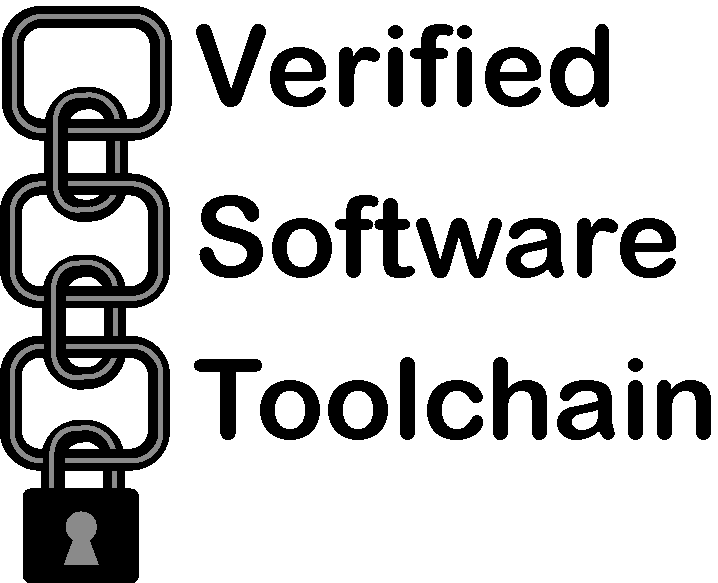
\includegraphics[width=.07\textwidth]{img/chain.png}};


      \draw (0.5,3) node [textstyle, anchor=west, draw=black, thick, minimum width=3cm,minimum height=0.5cm] (ml) {$\Zfield$};
      \draw (0,3) node [anchor=east] (shn) {Mid Level};

      \draw[thick,double, <->, >=implies] (ll.north) -- (ml.south);

      \draw (0.5,4) node [textstyle, anchor=west, draw=black, thick, minimum width=3cm,minimum height=0.5cm] (hl) {$\K$};
      \draw (0,4) node [anchor=east] (shn) {High Level};

      \draw[thick,double, <-, >=implies] (ml.north) -- (hl.south);
    \end{scope}
\end{tikzpicture}

  \caption{Structural construction of the proof}
  \label{tk:ProofStructure}
\end{figure}
